\documentclass{article}

\usepackage{amsmath} % math stuff
\usepackage{amssymb} % math stuff
\usepackage{array} % equations and stuff
\usepackage{bm} % bold math
%\usepackage{caption} % suppressed table numbering; incompatible with revtex, and longtable, I think
\usepackage{comment} % comment environment
%\usepackage{enumitem} % customization of enumeration, itemize, and description
\usepackage[T1]{fontenc} % font encoding for special characters, must also use scalable font package
\usepackage[margin=0.8in]{geometry} % paper sizes and margins (but be careful not to mess up pre-defined pages)
\usepackage{graphicx} % for graphics
%\usepackage{helvet} % default font is the helvetica postscript font
\usepackage{layouts} % print units like widths
\usepackage{lipsum} % lorem ipsum filler text
\usepackage{lmodern} % scalable font?
\usepackage{longtable} % multi-page tables
\usepackage{makecell} % specify line-breaks in table cells
\usepackage{mathrsfs} % math script font
\usepackage{mhchem} % easier chemical formula
\usepackage{microtype} % allows disabling of ligatures
%\usepackage{newcent} % new century schoolbook font
\usepackage{nicefrac}
\usepackage{numprint} % print and format (large) numbers
\usepackage{parskip} % removes paragraph indentation, and adjusts paragraph skip, as well as list items
\usepackage{pdfpages} % add pdf files as pages
%\usepackage{setspace} % adjust text spacing and indents
\usepackage{siunitx} % decimal alignment
\usepackage{subfigure} % divided figures
%\usepackage{tabu} % extra table options
\usepackage{textcomp} % symbols
\usepackage{threeparttablex} % better footnotes with longtable
\usepackage{titling} % title placement
\usepackage{ulem} % strikethrough text
%\usepackage{url} % superceded by hyperref
\usepackage{verbatim} % verbatim environment
\usepackage{xcolor} % colors and color boxes
\usepackage{xspace} % commands that don't eat up white space
\usepackage{hyperref} % links and page setup; should always come last

\hypersetup{
 bookmarks=true,
 colorlinks=true,
 citecolor=blue,
 linkcolor=blue,
 urlcolor=blue,
 pdfstartview={XYZ null null 1.0} % default open view is 100%
}

\DisableLigatures[f,t]{encoding = T1} % disable ff, fi, fl, tt ligatures, without f option, it also disables -- = endash
\renewcommand{\arraystretch}{2.0} % extra vertical space in tables

\begin{document}

\pagestyle{empty} % don't number pages

% custom title
\begin{center}
{\LARGE Express Riddler}

\vspace{0.15in}

{\Large 20 September 2019}
\end{center}


\section*{Riddle:}

This week, Riddler Nation needs your help designing its new credit card, appropriately named Riddler Express™---don't solve puzzles without it!

The logo consists of two overlapping circles with radius 1 inch, creating three distinct regions: one region that's shared between the two circles, and two regions that are part of one circle, but not the other.

\begin{center}
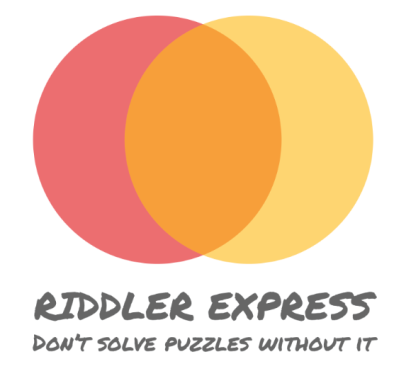
\includegraphics[width=3in]{Riddler_express_card.png}
\end{center}

Because the Riddler Express™ card is for the mathematically inclined, its parent company has issued a corporate mandate regarding symmetry.
In particular, the areas of all three regions must be \textit{exactly} the same.
If that's the case, how far apart must the centers of the two circles be?

\textbf{Extra Credit}: If you symmetrically arrange \textit{three} circles of radius 1, you have seven distinct regions.
How far apart should the centers of the circles be such that the areas of the largest and smallest of the seven regions are as close to equivalent as possible?

\section*{Solution:}

The following diagram illustrates the quantities used to solve this riddle.

\begin{center}
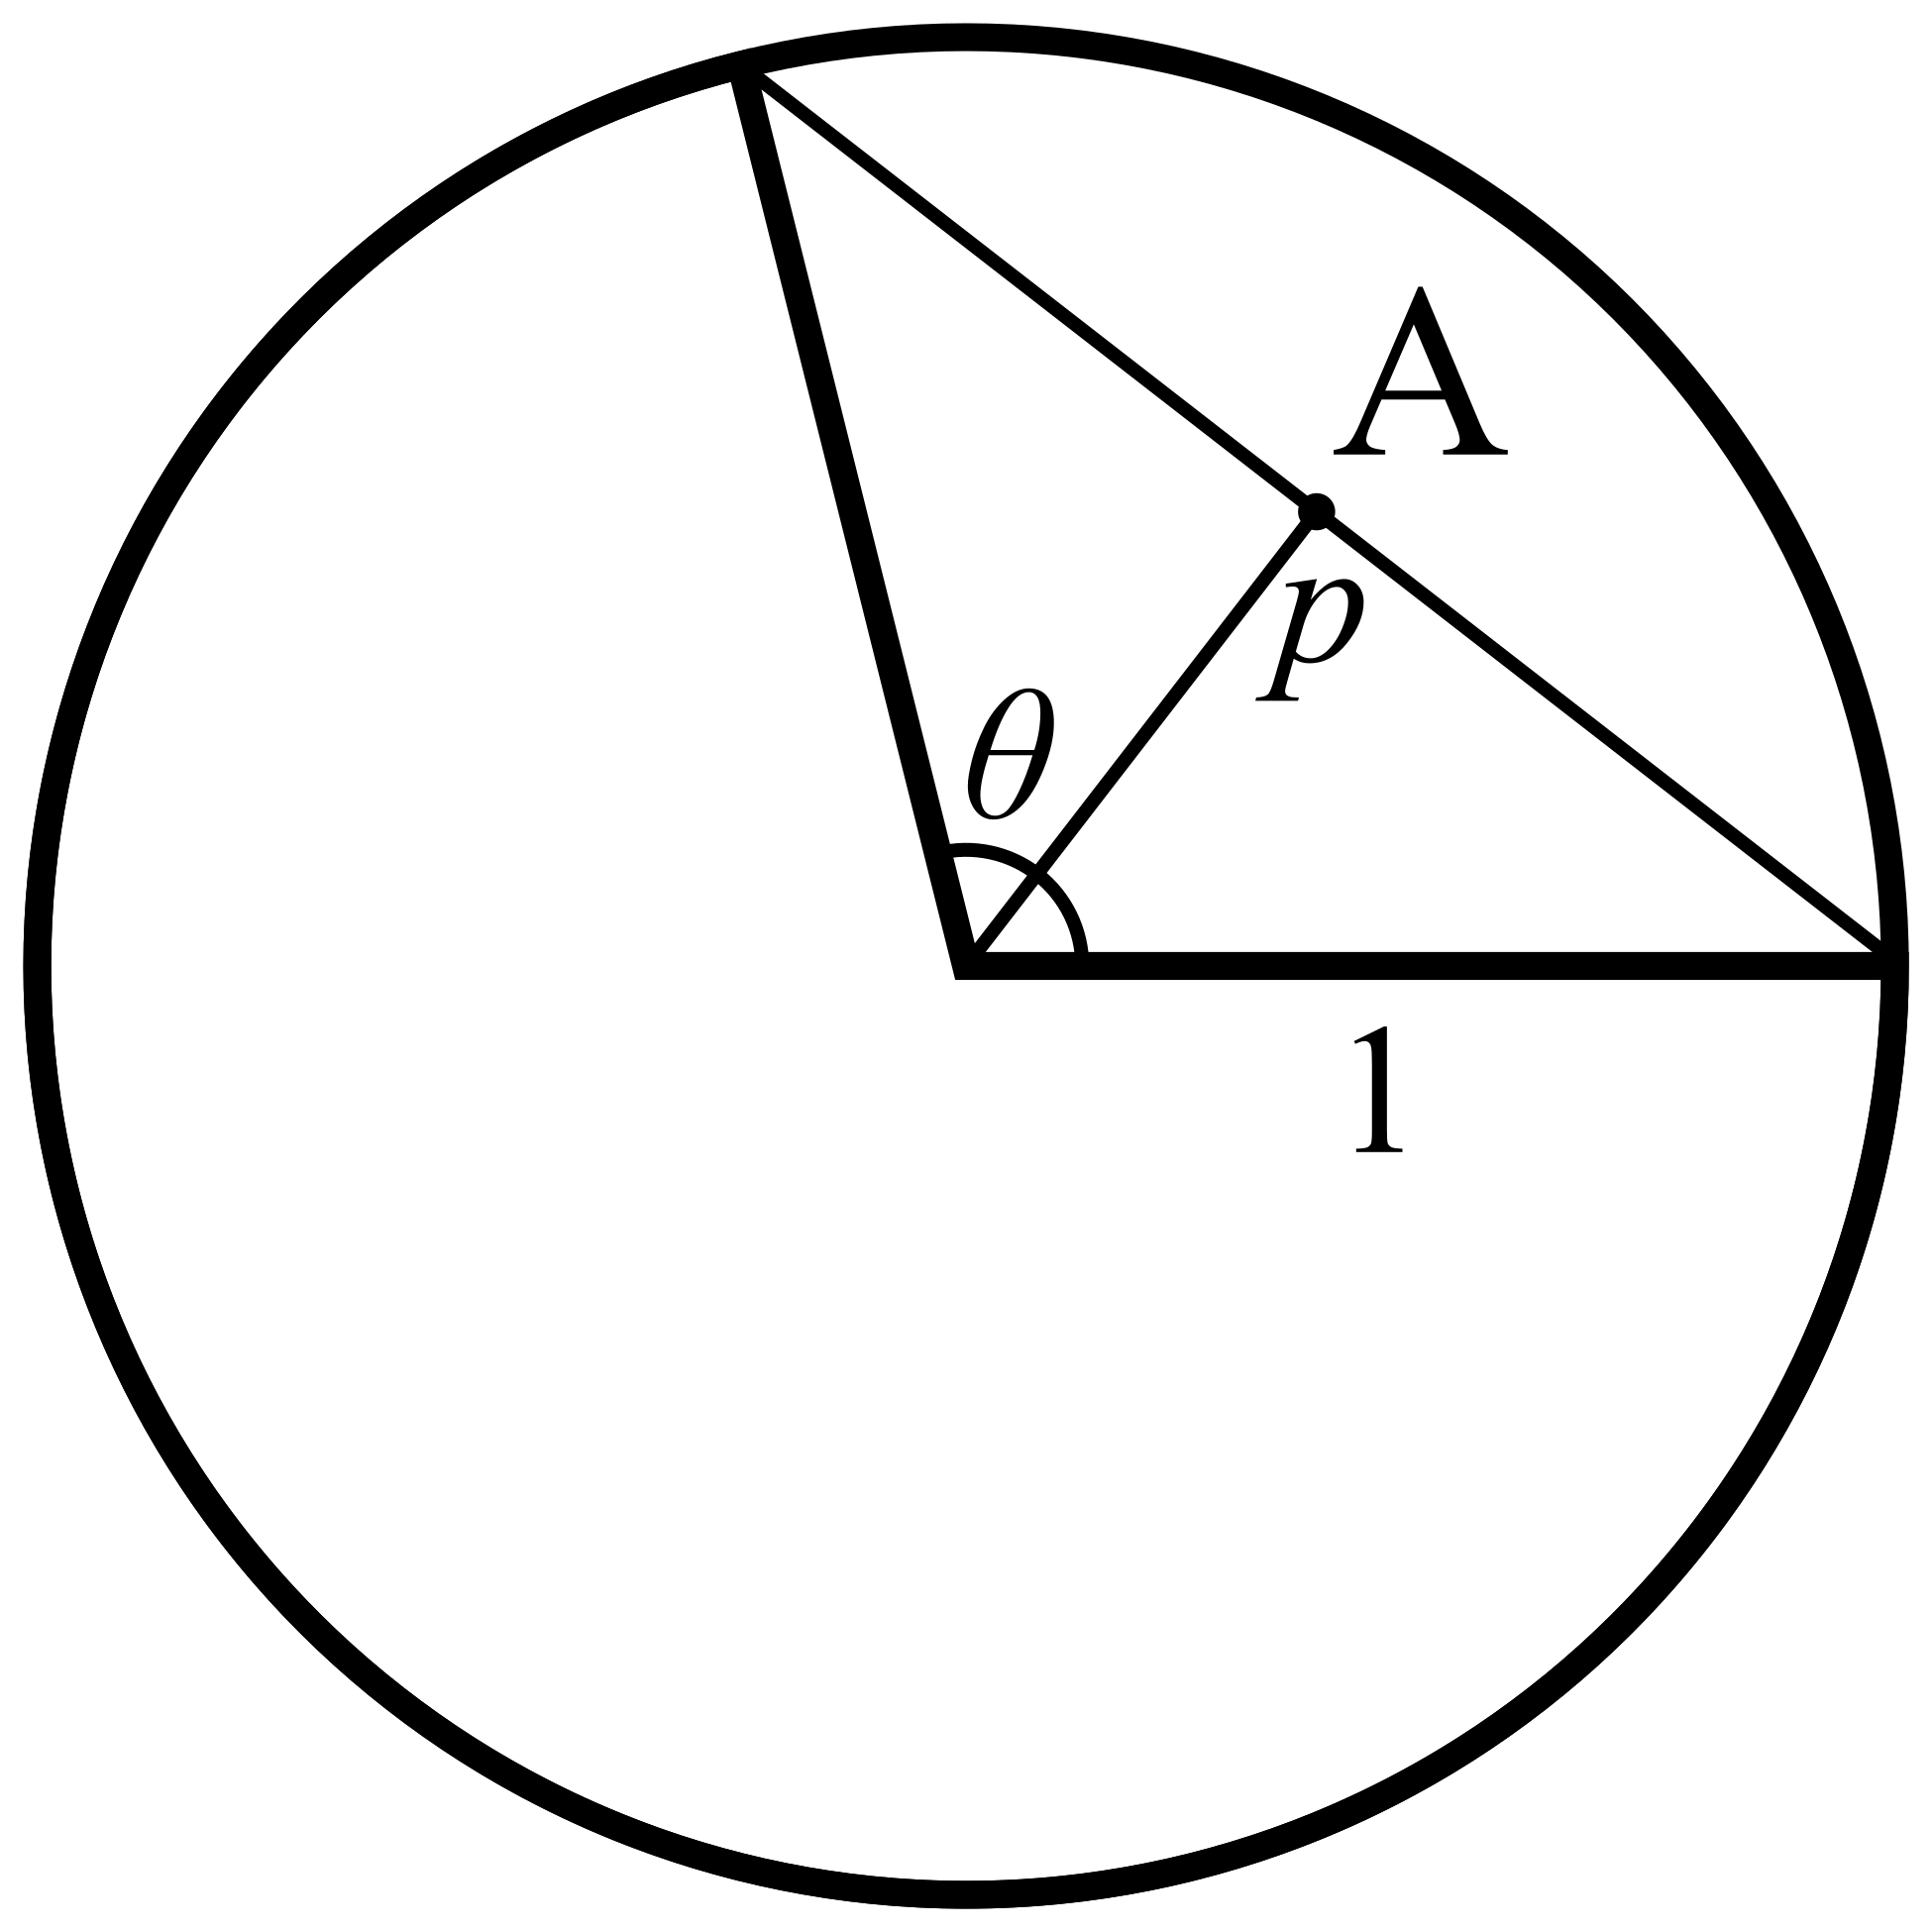
\includegraphics[width=2in]{circle_diagram.png}
\end{center}

The quasi-lune area $A$ represents half of the overlapping region.
With a radius of 1, the area of each circle is $\pi1^{2}=\pi$.
Then the area of the overlapping region is $\nicefrac{\pi}{2}$, and the area of $A$ is $\nicefrac{\pi}{4}$.
The area can be solved from by subtracting the area of the triangle $A_{t}$ from the area of the arc $A_{a}$, both determined by the angle $\theta$:

\begin{align*}
A = \frac{\pi}{4}  &= A_{a}-A_{t} \\
                   &= \pi\left(\frac{\theta}{2\pi}\right)-\frac{\sin\theta}{2}
\end{align*}

which gives

\[
\theta-\sin\theta=\frac{\pi}{2}
\]

This has the unique solution $\theta\approx2.3099$.
Now with the angle determined, the distance between the circles' centers can be calculated.
With the point $p$ at the midpoint of the connecting line, it is also located halfway between the two circles' centers.
Therefore the centers are separated by twice the distance $\overline{op}$ (with point $o$ as the origin of the unit circle):

\begin{align*}
2\overline{op} &= 2\sqrt{\left(0-\frac{1+\cos\theta}{2}\right)^{2}+\left(0-\frac{\sin\theta}{2}\right)^{2}} \\
              &= \sqrt{2+2\cos\theta}
\end{align*}

This has the (approximate) solution
\fcolorbox{red}{white}{\bf 0.8079}\,.



\end{document}